% !TeX spellcheck = en_US
% !TeX encoding = UTF-8
\documentclass[10pt,aspectratio=1610,xcolor={usenames,dvipsnames,table}]{beamer}
\mode<presentation>
\usepackage[T1]{fontenc}
\usepackage[utf8]{inputenc}
\usepackage[english]{babel}
\usepackage{lmodern}
\usepackage[babel,style=english,english=american]{csquotes}
\usepackage{mathabx}
\usepackage{latexsym}
\usepackage{graphicx}
\usepackage{multicol}
\usepackage{multirow}
\usepackage[gen]{eurosym}
\usepackage{pgfpages}
\usepackage{xspace}
\usepackage{appendixnumberbeamer}
\usepackage[binary-units]{siunitx}
\usepackage{tabu}
\usepackage{graphicx}
\usepackage{pgfgantt}
%\usepackage{biblatex}

%\setcounter{tocdepth}{2}

%\usetheme[numbering=counter,progressbar=frametitle]{metropolis}
%\usetheme[numbering=none]{metropolis}
\usetheme[sectionpage=none,subsectionpage=none,numbering=counter,progressbar=none]{metropolis}

\title{Software Development Project}
\subtitle{Basic Navigation Test Analysis}
\titlegraphic{
\includegraphics[width=5cm]{gfx/logo}}
\author{Wei-Chan Hsu, Torsten Jandt, Ramesh Kumar, Danning Wang}
\date{June 26, 2017}

\setbeamertemplate{caption}{\raggedright\insertcaption\par}



\setbeamerfont{footnote}{size=\tiny}

\begin{document}

\begin{frame}[noframenumbering,plain]
\titlepage
\end{frame}


\begin{frame}{Class Diagram}
    \begin{center}
        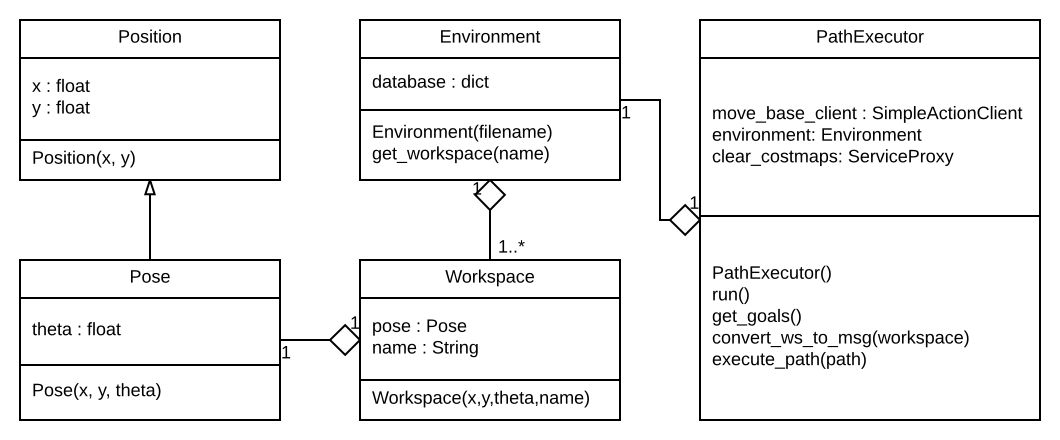
\includegraphics[width=\linewidth,height=0.9\textheight,keepaspectratio]{gfx/01.pdf}
    \end{center}
\end{frame}


\begin{frame}{Sequence Diagram}
    \begin{center}
        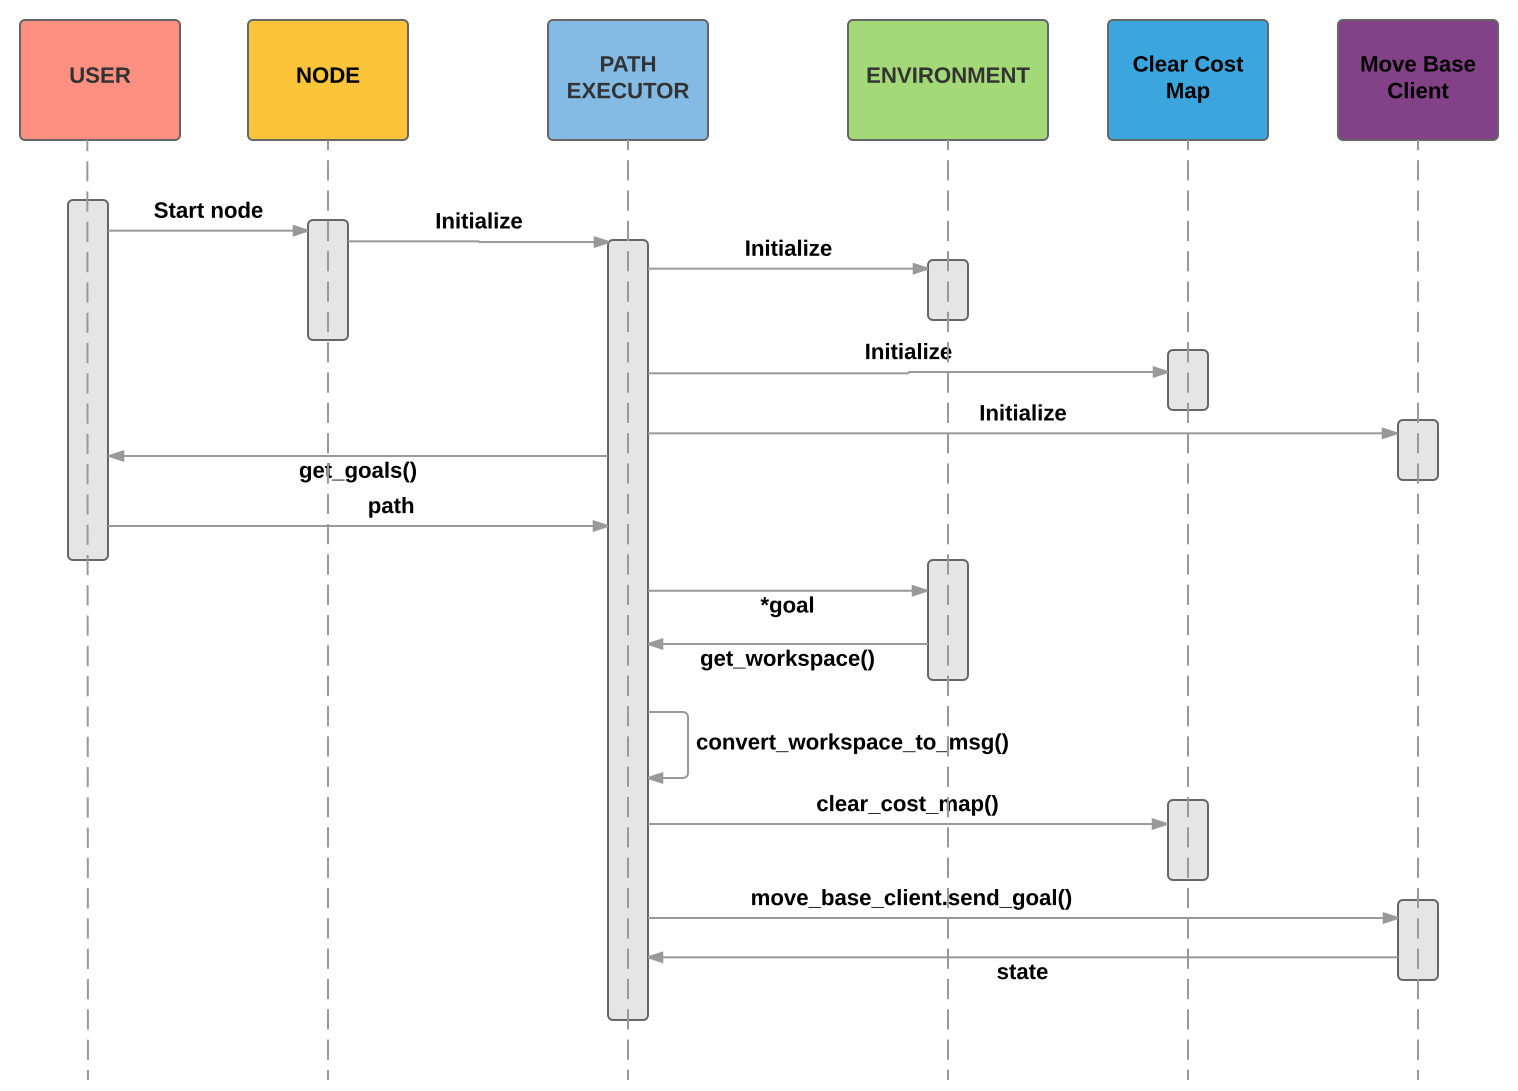
\includegraphics[width=\linewidth,height=0.9\textheight,keepaspectratio]{gfx/02.pdf}
    \end{center}
\end{frame}


\end{document}